\documentclass[a4paper,twoside,12pt,nochapterprefix]{scrbook}


\usepackage{amsmath,amssymb,amsthm}
\usepackage[footnotesize,sl,SL,hang,tight]{subfigure}  % helpful package for aligning figures next to each other
\usepackage{longtable} % tables over several pages
\usepackage[font={small,sl},hang,labelfont=bf]{caption} % configure captions
\usepackage{booktabs} % publication quality tables for LaTeX
%\usepackage{showkeys} % shows the labels above the references for easier development

\ifpdfoutput{%
	\usepackage[pdftex]{graphicx}
	\usepackage[]{pdfpages} %for including full pdf pages
}{%
	\usepackage{graphicx}
}
\usepackage{epstopdf}
\epstopdfsetup{update} % only regenerate pdf files when eps file is newer

\usepackage{rotating} % rotate figures

\usepackage[headinclude]{scrpage2}

% Font packages:
\usepackage{times}
\usepackage{helvet}   % sets sans serif font
\usepackage[T1]{fontenc}

%PDF hyperref config
\ifpdfoutput{%
	\usepackage[pdftex,
		a4paper,
		bookmarks,
		bookmarksopen=true,
		bookmarksnumbered=true,
		pdfauthor={Andreas Ziegler},       % FILL THIS IN PROPERLY
		pdftitle={Robust	object	tracking	in	3D	by	fusing	ultra-wideband	and	vision},   % FILL THIS IN PRPERLY
		colorlinks,
		linkcolor=black,
		citecolor=black,
		filecolor=black,
		urlcolor=black,
		anchorcolor=black,
		menucolor=black,
		breaklinks=true,
		pageanchor=true,
		plainpages=false,
		pdfpagelabels=true]{hyperref}
}{}

\ifpdfoutput{%
	\pdfcompresslevel=9
	\pdfoutput=1
	\DeclareGraphicsExtensions{.pdf,.png}
}{}

\bibliographystyle{acmsiggraph}



% A4
%
\topmargin -0.5in
\textheight 9.3in
\textwidth 6.3in
\oddsidemargin 0.18in
\evensidemargin -0.22in
\parskip 0.1in
\parindent 0in

\renewcommand{\arraystretch}{1.5}
\renewcommand{\baselinestretch}{1}

% !TEX root = ../thesis.tex

% TO DO search symbol
\newcommand{\TODO}{\mbox{\large\bf TO DO}}
\newcommand{\REFR}{\mbox{\large\bf REFR}}

%  Terminates current page and paragraph, makes sure next page starts on
%  an odd-number, and generates a completely blank page, without page markers,
%  if necessary.
\newcommand{\clearemptydoublepage}{\newpage{\pagestyle{empty}\cleardoublepage}}


% !TEX root = ../thesis.tex

% Stripped from acm siggraph bst and cls
\makeatletter

% no labels in bibliography.
\def\@biblabel#1{}

\newlength{\bibhang}
\setlength{\bibhang}{1em}

% Change in-bibliography biberence style
\def\thebibliography#1{%
  \section*{%
    \bibname\@mkboth{\sl\uppercase{\bibname}}{\sl\uppercase{\bibname}}}
  \list{\relax}{\setlength{\labelsep}{0em}
                \setlength{\itemindent}{-\bibhang}
                \setlength{\leftmargin}{\bibhang}}
  \def\newblock{\hskip .11em plus .33em minus .07em}
  \sloppy\clubpenalty4000\widowpenalty4000
  \sfcode`\.=1000\relax}

% Not sure what this does...
%\def\@citex[#1]#2{\if@filesw\immediate\write\@auxout{\string\citation{#2}}\fi
%  \def\@citea{}\@cite{\@for\@citeb:=#2\do
%    {\@citea\def\@citea{; }\@ifundefined
%      {b@\@citeb}{{\bf ?}\@warning
%      {Citation '\@citeb' on page \thepage \space undefined}}%
%{\csname b@\@citeb\endcsname}}}{#1}}

% Change in-document citation styles
\let\@internalcite\cite
\def\cite{\def\citename##1{##1}\@internalcite}
\def\shortcite{\def\citename##1{}\@internalcite}

\makeatother


\begin{document}

%% Define leading chapter pages
%
% !TEX root = ../thesis.tex

\addtokomafont{chapter}{\setlength{\parskip}{190pt}}   % SEVERE HACK to keep spacing to chapter art work
%\addtokomafont{chapter}{\rmfamily}        % remove this if you prefer sans-serif section titles
%\addtokomafont{section}{\rmfamily}        % remove this if you prefer sans-serif section titles
%\addtokomafont{subsection}{\rmfamily}     % remove this if you prefer sans-serif section titles
%\addtokomafont{subsubsection}{\rmfamily}  % remove this if you prefer sans-serif section titles
%\addtokomafont{paragraph}{\rmfamily}      % replace by \sffamily if you prefer sans-serif para titles
\addtokomafont{paragraph}{\sffamily}

\def\mychpstyleintl{%
{\noindent\setlength{\tabcolsep}{0pt}\setlength{\arrayrulewidth}{2pt}%
\begin{tabular}{c}
\\[100pt]
\begin{tabular}{lr}
\begin{tabular}{p{0.6\linewidth}}
\\
\end{tabular}
&
\begin{tabular}{p{0.4\linewidth}}
\rightline{{%
\sffamily%
\fontseries{bx}%
\fontshape{n}%
\fontsize{100}{120}%choose baselineskip to be 1.2 times font size
\selectfont
\thechapter}}
\end{tabular}
\end{tabular}\\[300pt]
\end{tabular}
}}

\newpagestyle{mychapterpagestyle}{{\protect\mychpstyleintl}{\protect\mychpstyleintl}}{}
\newpagestyle{myappendixpagestyle}{{\protect\mychpstyleintl}{\protect\mychpstyleintl}}{}
%%

%% macros e.g.
\newcommand{\mfytext}[0]{my fancy text}

%refs
\newcommand{\chpref}[1]{Chapter \ref{#1}}
\newcommand{\secref}[1]{Section \ref{#1}}
%\newcommand{\equref}[1]{Equation \ref{#1}} %better use builtin \eqref{}
\newcommand{\figref}[1]{Figure \ref{#1}}
\newcommand{\tabref}[1]{Table \ref{#1}}
\newcommand{\apxref}[1]{Appendix \ref{#1}}
%%

%% Replace this by your own design of a title page
%
%\title{Thesis Title}
%\author{My Name}
%\date{September 2042}
%\maketitle
%\clearemptydoublepage
% --- selfmade version ----
\begin{titlepage}
	\topmargin 1.0cm
	\oddsidemargin 0.0cm
	\evensidemargin 0.0cm
	%\textwidth 6.5in
	\centering
	\Huge
	\vspace{3.0cm}
	\textbf{\textsf{Robust object tracking in 3D by fusing ultra-wideband and vision}} \\[2.0cm]
	\includegraphics*[width=0.8\textwidth]{figures/teaser} \\ % TITLE IMAGE - replace by attractive and representative images from your thesis
	\vspace{3cm}
	\sffamily
	\Large
	Andreas Ziegler
	\\[0.8cm]
	\large
	Semester Project % Bachelor Thesis
	\\
	June 2016
	\\[1.3cm]
	\emph{Supervisors:}\\
	Benjamin Hepp\\ 					% The name of the thesis supervisor
	Prof.\ Dr.\ Otmar Hilliges\\		% The supervising professor
	Prof.\ Dr.\ Luv Van Gool
	\vfill
	\includegraphics*[height=0.8cm]{figures/eth_logo_kurz_pos.eps} \hfill
	\includegraphics*[height=0.8cm]{figures/logo-ait}
	\vspace{3.4cm}
\end{titlepage}
\clearemptydoublepage
%%

\pagenumbering{roman}
\setcounter{page}{1}

% !TEX root = ../thesis.tex

\chapter*{Abstract}
\paragraph*{Motivation}
Object tracking is an important part for many applications especially for robotic systems interacting with humans.

\paragraph*{Problem statement}
\ac{UWB} systems as well as vision based object trackers are widely known and used. Both of the systems have their advantages and disadvantages. \ac{UWB} systems can provide the location of an object in 3D with an accuracy of approximate $10\textit{cm}$ whereas vision based object trackers can only provide the location of an object in 2D pixel coordinates but with a more precise accuracy than \ac{UWB} systems.

\paragraph*{Approach}
So why not combine these two sources of information? Exactly this concept should be developed and evaluated in this semester project. The 3D position measured by the UWB system should be fused with the 2D pixel coordinates of a visual object tracker with an \ac{EKF}. A re-detection mechanism for the visual tracker should be implemented in addition to increase the usability as well as the stability of the system.

\paragraph*{Result}
The proposed system shows a significantly better accuracy compared with the 3D positions measured by the \ac{UWB} system. This proof of concept enables to apply this system to a wide range of applications and also allows further extensions.
\cleardoublepage
%\chapter*{Zusammenfassung}

%Diese Arbeit besch�ftigt sich mit der Entwicklung einer neuartigen Beispielausarbeitung. Wir untersuchen die Anforderungen, die sich f�r eine allgemeine Vorlage ergeben, die innerhalb der \LaTeX-Textverarbeitungsumgebung verwendet werden kann. (Und so weiter und so fort\dots) Die Zusammenfassung sollte nicht l�nger als eine halbe Textseite sein!


%-----------------------------------------------------------------------------------------------
%include task description here:
\cleardoublepage
%\includegraphics[viewport=3cm 0cm 20cm 27.5cm]{task_description} %better use includepdf below!
%\includepdf{task_description}
\cleardoublepage
%-----------------------------------------------------------------------------------------------

%include acknowledgment here:
%\include{./chapters/acknowledgment}

\tableofcontents

\cleardoublepage
\phantomsection
\addcontentsline{toc}{chapter}{List of Figures}
\listoffigures

\cleardoublepage
\phantomsection
\addcontentsline{toc}{chapter}{List of Tables}
\listoftables
\cleardoublepage

\pagenumbering{arabic}
\renewcommand*{\chapterpagestyle}{mychapterpagestyle}
\renewcommand*{\chapterformat}{} % show chapter titles only (no numbers)
% \setchapterpreamble[o]{...}  unfortunately does not move the \chapter output downwards

% ---- MAIN PART ----

% !TEX root = ../thesis.tex

% set counter to n-1:
\setcounter{chapter}{0}

\chapter{Introduction}

Object tracking is an important building block for	many interactive systems, especially for robotic systems interacting with humans. State-of-the-art robust approaches detect and recognize a small number of pre-defined	object types like humans,	birds	or cars. For	many applications tracking of arbitrary objects	is desirable, i.e. a bottle,	a hand, an animal, a face etc. Online visual tracking deals with the	challenging	task of tracking an object based on an initial bounding box in an image. This faces the fundamental problem of very limited labeled data and as a consequence any such tracking approach has to balance plasticity and drift, in particular when an object	should	be re-detected after loss of tracking. In this semester project a new approach is proposed. A fusion of \ac{UWB} and visual	measurements to track an object in 3D by fusing both modalities in a principled manner.

This semester project focuses on visual tracking with correlation filters. This is typically susceptible to drift and has low accuracy in the radial direction. The aim is to compensate for this with an additional existing sensor modality based on multilateration with \ac{UWB} signals. A single tracker consists of multiple \ac{UWB} units that track a single \ac{UWB} unit on the target, providing a 3D position and covariance of the target. Because of the arrangement of the \ac{UWB} units the tangential accuracy of the \ac{UWB} position is relatively low. The visual tracker will provide a 2D measurement and a confidence. Together both observations should be fused in a principled manner using an \ac{EKF} that will combine the strength of both approaches.
% !TEX root = ../thesis.tex

% set counter to n-1:
\setcounter{chapter}{1}

\chapter{Related Work}

Lorem ipsum dolor sit amet, consectetuer adipiscing elit, sed diam nonummy nibh euismod tincidunt ut laoreet dolore magna aliquam erat volutpat. Ut wisi enim ad minim veniam, quis nostrud exerci tation ullamcorper suscipit lobortis nisl ut aliquip ex ea commodo consequat. Duis autem vel eum iriure dolor in hendrerit in vulputate velit esse molestie consequat, vel illum dolore eu feugiat nulla facilisis at vero et accumsan et iusto odio dignissim qui.

Sample references are~\cite{Zwicker04Perspective} and~\cite{Altman89QuaternionScandal}.

\section{Appearance Modeling}


Lorem ipsum dolor sit amet, consectetuer adipiscing elit, sed diam nonummy nibh euismod tincidunt ut laoreet dolore magna aliquam erat volutpat. Ut wisi in hendrerit in vulputate velit esse molestie consequat, vel illum dolore eu feugiat nulla facilisis at vero et accumsan et iusto odio dignissim qui blandit praesent luptatum zzril delenit augue duis dolore te feugait nulla facilisi. Lorem ipsum dolor sit amet, consectetuer adipiscing elit, sed diam 

\subsection{Taxonomy}

Lorem ipsum dolor sit amet, consectetuer adipiscing elit, sed diam nonummy nibh euismod tincidunt ut laoreet dolore magna aliquam erat volutpat. Ut wisi enim ad minim veniam, quis nostrud exerci tation ullamcorper suscipit lobortis nisl ut aliquip ex ea commodo consequat. Duis autem vel eum iriure dolor in hendrerit in vulputate velit esse molestie consequat, vel illum dolore eu feugiat nulla facilisis at vero et accumsan et iusto odio dignissim qui blandit praesent luptatum zzril delenit augue duis dolore te feugait nulla facilisi. Lorem ipsum dolor sit amet, consectetuer adipiscing elit, sed diam 
in hendrerit in vulputate velit esse molestie consequat, vel illum dolore eu feugiat nulla facilisis at vero et accumsan et iusto odio dignissim qui blandit praesent luptatum zzril delenit augue duis dolore te feugait nulla facilisi. Lorem ipsum dolor sit amet, consectetuer adipiscing elit, sed diam 

in hendrerit in vulputate velit esse molestie consequat, vel illum dolore eu feugiat nulla facilisis at vero et accumsan et iusto odio dignissim qui blandit praesent luptatum zzril delenit augue duis dolore te feugait nulla facilisi. Lorem ipsum dolor sit amet, consectetuer adipiscing elit, sed diam 
in hendrerit in vulputate velit esse molestie consequat, vel illum dolore eu feugiat nulla facilisis at vero et accumsan et iusto odio dignissim qui blandit praesent luptatum zzril delenit augue duis dolore te feugait nulla facilisi. Lorem ipsum dolor sit amet, consectetuer adipiscing elit, sed diam 

\subsection{Appearance Models}


Lorem ipsum dolor sit amet, consectetuer adipiscing elit, sed diam nonummy nibh euismod tincidunt ut laoreet dolore magna aliquam erat volutpat. Ut wisi enim ad minim veniam, quis nostrud exerci tation ullamcorper suscipit lobortis nisl ut aliquip ex ea commodo consequat. Duis autem vel eum iriure dolor in hendrerit in vulputate velit esse molestie consequat, vel illum dolore eu feugiat nulla facilisis at vero et accumsan et iusto odio dignissim qui blandit praesent luptatum zzril delenit augue duis dolore te feugait nulla facilisi. Lorem ipsum dolor sit amet, consectetuer adipiscing elit, sed diam 

Lorem ipsum dolor sit amet, consectetuer adipiscing elit, sed diam nonummy nibh euismod tincidunt ut laoreet dolore magna aliquam erat volutpat. Ut wisi enim ad minim veniam, quis nostrud exerci tation ullamcorper suscipit lobortis nisl ut aliquip ex ea commodo consequat. Duis autem vel eum iriure dolor in hendrerit in vulputate velit esse molestie consequat, vel illum dolore eu feugiat nulla facilisis at vero et accumsan et iusto odio dignissim qui blandit praesent luptatum zzril delenit augue duis dolore te feugait nulla facilisi. Lorem ipsum dolor sit amet, consectetuer adipiscing elit, sed diam 

\section{Human Skin Rendering}


Lorem ipsum dolor sit amet, consectetuer adipiscing elit, sed diam nonummy nibh euismod tincidunt ut laoreet dolore magna aliquam erat volutpat. Ut wisi enim ad minim veniam, quis nostrud exerci tation ullamcorper suscipit lobortis nisl ut aliquip ex ea commodo consequat. Duis autem vel eum iriure dolor in hendrerit in vulputate velit esse molestie consequat, vel illum dolore eu feugiat nulla facilisis at vero et accumsan et iusto odio dignissim qui blandit praesent luptatum zzril delenit augue duis dolore te feugait nulla facilisi. Lorem ipsum dolor sit amet, consectetuer adipiscing elit, sed diam 

in hendrerit in vulputate velit esse molestie consequat, vel illum dolore eu feugiat nulla facilisis at vero et accumsan et iusto odio dignissim qui blandit praesent luptatum zzril delenit augue duis dolore te feugait nulla facilisi. Lorem ipsum dolor sit amet, consectetuer adipiscing elit, sed diam 
Lorem ipsum dolor sit amet, consectetuer adipiscing elit, sed diam nonummy nibh euismod tincidunt ut laoreet dolore magna aliquam erat volutpat. Ut wisi enim ad minim veniam, quis nostrud exerci tation ullamcorper suscipit lobortis nisl ut aliquip ex ea commodo consequat. Duis autem vel eum iriure dolor in hendrerit in vulputate velit esse molestie consequat, vel illum dolore eu feugiat nulla facilisis at vero et accumsan et iusto odio dignissim qui blandit praesent luptatum zzril delenit augue duis dolore te feugait nulla facilisi. Lorem ipsum dolor sit amet, consectetuer adipiscing elit, sed diam 
in hendrerit in vulputate velit esse molestie consequat, vel illum dolore eu feugiat nulla facilisis at vero et accumsan et iusto odio dignissim qui blandit praesent luptatum zzril delenit augue duis dolore te feugait nulla facilisi. Lorem ipsum dolor sit amet, consectetuer adipiscing elit, sed diam 
Lorem ipsum dolor sit amet, consectetuer adipiscing elit, sed diam nonummy nibh euismod tincidunt ut laoreet dolore magna aliquam erat volutpat. Ut wisi enim ad minim veniam, quis nostrud exerci tation ullamcorper suscipit lobortis nisl ut aliquip ex ea commodo consequat. Duis autem vel eum iriure dolor in hendrerit in vulputate velit esse molestie consequat, vel illum dolore eu feugiat nulla facilisis at vero et accumsan et iusto odio dignissim qui blandit praesent luptatum zzril delenit augue duis dolore te feugait nulla facilisi. Lorem ipsum dolor sit amet, consectetuer adipiscing elit, sed diam 

in hendrerit in vulputate velit esse molestie consequat, vel illum dolore eu feugiat nulla facilisis at vero et accumsan et iusto odio dignissim qui blandit praesent luptatum zzril delenit augue duis dolore te feugait nulla facilisi. Lorem ipsum dolor sit amet, consectetuer adipiscing elit, sed diam 
Lorem ipsum dolor sit amet, consectetuer adipiscing elit, sed diam nonummy nibh euismod tincidunt ut laoreet dolore magna aliquam erat volutpat. Ut wisi enim ad minim veniam, quis nostrud exerci tation ullamcorper suscipit lobortis nisl ut aliquip ex ea commodo consequat. Duis autem vel eum iriure dolor in hendrerit in vulputate velit esse molestie consequat, vel illum dolore eu feugiat nulla facilisis at vero et accumsan et iusto odio dignissim qui blandit praesent luptatum zzril delenit augue duis dolore te feugait nulla facilisi. Lorem ipsum dolor sit amet, consectetuer adipiscing elit, sed diam 

% !TEX root = ../thesis.tex

\chapter{Your Central Work}

Lorem ipsum dolor sit amet, consectetuer adipiscing elit, sed diam nonummy nibh euismod tincidunt ut laoreet dolore magna aliquam erat volutpat. Ut wisi enim ad minim veniam, quis nostrud exerci tation ullamcorper suscipit lobortis nisl ut aliquip ex ea commodo consequat. Duis autem vel eum iriure dolor in hendrerit in vulputate velit esse molestie consequat, vel illum dolore eu feugiat nulla facilisis at vero et accumsan et iusto odio dignissim qui blandit.

\section{First Section}

Lorem ipsum dolor sit amet, consectetuer adipiscing elit, sed diam nonummy nibh euismod tincidunt ut laoreet dolore magna aliquam erat volutpat. Ut wisi enim ad minim veniam, quis nostrud exerci tation ullamcorper suscipit lobortis nisl ut aliquip ex ea commodo consequat. Duis autem vel eum iriure dolor in hendrerit in vulputate velit esse molestie consequat, vel illum dolore eu feugiat nulla facilisis at vero et accumsan et iusto odio dignissim qui blandit praesent luptatum zzril delenit augue duis dolore te feugait nulla facilisi. Lorem ipsum dolor sit amet, consectetuer adipiscing elit, sed diam  praesent luptatum zzril delenit augue duis dolore te feugait nulla facilisi. Lorem ipsum dolor sit amet, consectetuer adipiscing elit, sed diam nonummy nibh euismod tincidunt ut laoreet dolore magna aliquam erat volutpat. Ut wisi enim ad minim veniam, quis nostrud exerci tation ullamcorper suscipit lobortis nisl ut aliquip ex ea commodo consequat. Duis autem vel eum iriure dolor in hendrerit in vulputate velit esse molestie consequat, vel illum dolore eu feugiat nulla facilisis at vero et accumsan et iusto odio dignissim qui blandit.

Delenit augue duis dolore te feugait nulla facilisi. Lorem ipsum dolor sit amet, consectetuer adipiscing elit, sed diam  praesent luptatum zzril delenit augue duis dolore te feugait nulla facilisi. Lorem ipsum dolor sit amet, consectetuer adipiscing elit, sed diam nonummy nibh euismod tincidunt ut laoreet dolore magna aliquam erat volutpat. Ut wisi enim ad minim veniam, quis nostrud exerci tation ullamcorper suscipit lobortis nisl ut aliquip ex ea commodo consequat. Duis autem vel eum iriure dolor in hendrerit in vulputate velit esse molestie consequat, vel illum dolore eu feugiat nulla facilisis at vero et accumsan et iusto odio dignissim qui blandit.

\subsection{Fist Subsection}

Lorem ipsum dolor sit amet, consectetuer adipiscing elit, sed diam nonummy nibh euismod tincidunt ut laoreet dolore magna aliquam erat volutpat. Ut wisi enim ad minim veniam, quis nostrud exerci tation ullamcorper suscipit lobortis nisl ut aliquip ex ea commodo consequat. Duis autem vel eum iriure dolor in hendrerit in vulputate velit esse molestie consequat, vel illum dolore eu feugiat nulla facilisis at vero et accumsan et iusto odio dignissim qui blandit praesent luptatum zzril delenit augue duis dolore te feugait nulla facilisi. Lorem ipsum dolor sit amet, consectetuer adipiscing elit, sed diam 

\subsection{Another Subsection}

\begin{table}
    \centering
    \begin{tabular}{|l|p{0.4\linewidth}|}
    \hline
    \emph{Quant.} & \emph{Ingredient}\\
    \hline
		200g &Wei{\ss}mehl\\
		1/4  &Packung Frischhefe\\
		4EL  &lauwarme Milch\\
		4EL  &�l\\
		1TL  &Zucker\\
		1TL  &Salz\\
		&lauwarmes Wasser\\
    \hline
    \end{tabular}
    \caption[Flammkuchenteig]{Flammkuchenteig. The ingredients have to be carefully chosen.\label{tab:mytable}}
\end{table}
%
Lorem ipsum dolor sit amet, consectetuer adipiscing elit, sed diam nonummy nibh euismod tincidunt ut laoreet dolore magna aliquam erat volutpat. Ut wisi enim ad minim veniam, quis nostrud exerci tation ullamcorper suscipit lobortis nisl ut aliquip ex ea commodo consequat, see Table~\ref{tab:mytable}. Duis autem vel eum iriure dolor in hendrerit in vulputate velit esse molestie consequat, vel illum dolore eu feugiat nulla facilisis at vero et accumsan et iusto odio dignissim qui blandit praesent luptatum zzril delenit augue duis dolore te feugait nulla facilisi. Lorem ipsum dolor sit amet, consectetuer adipiscing elit, sed diam,
see Figure~\ref{fig:voldiff}~(a).
%
\begin{figure}
    \centering
    \setlength{\tabcolsep}{0.0130\linewidth}
    \begin{tabular}{@{}cc@{}}
    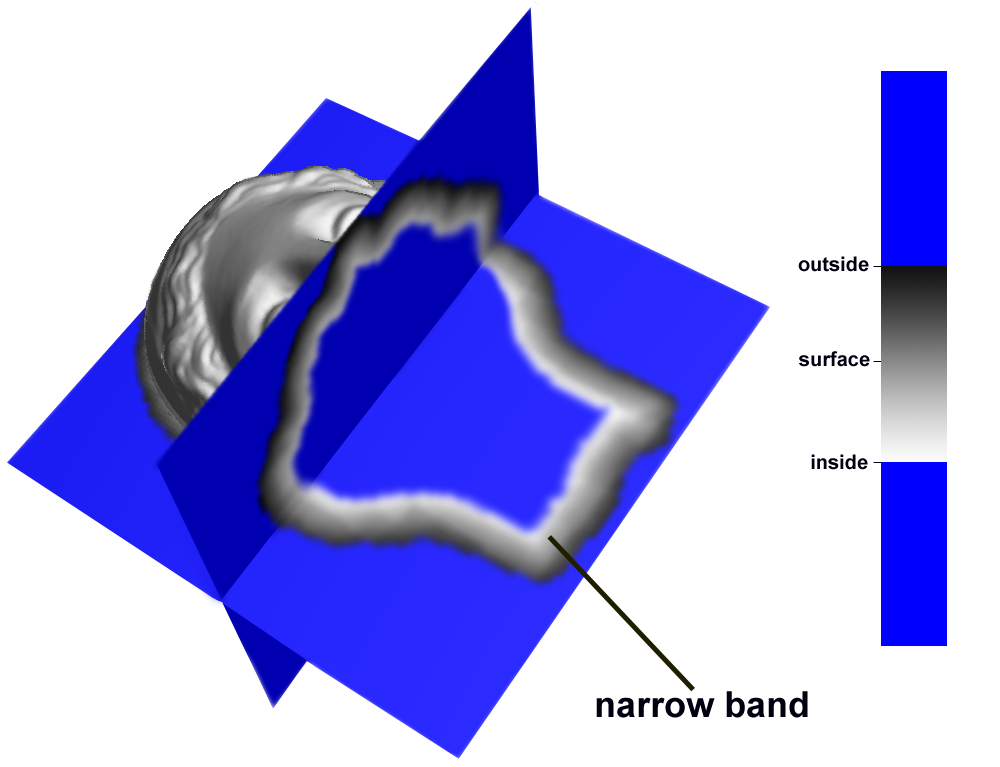
\includegraphics[width=0.487\linewidth]{figures/IgeaNarrowBand}&
    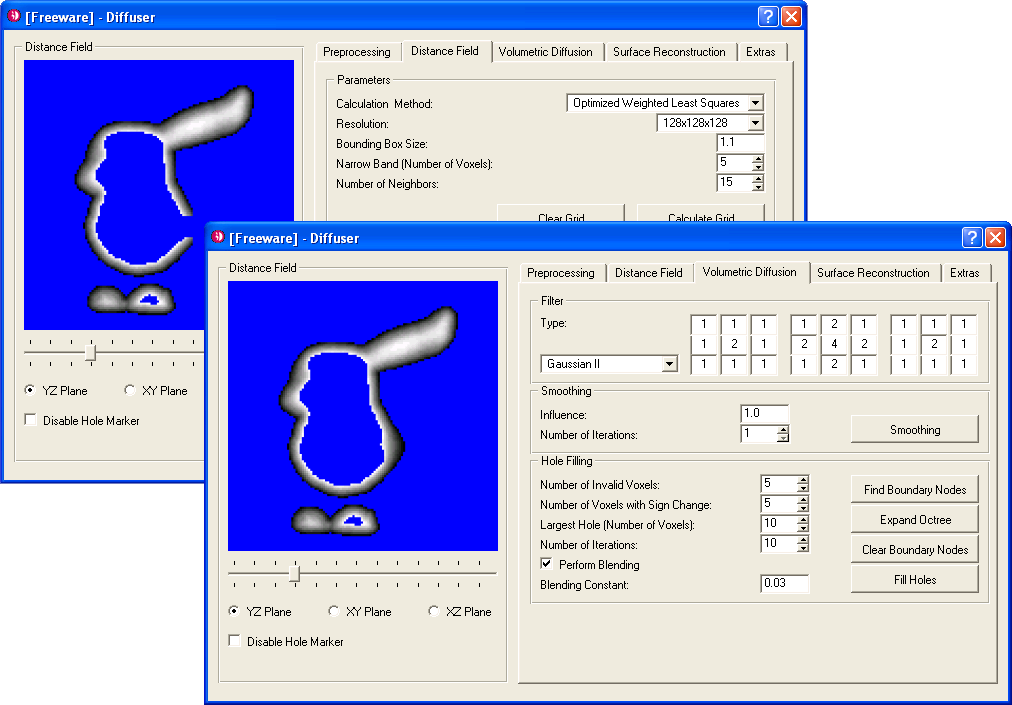
\includegraphics[width=0.487\linewidth]{figures/voldiff_ui}\\
    (a)&(b)\\
    \end{tabular}
    \caption[Volumetric diffusion]{Volumetric diffusion.
    	  \textup{(a)} Slices of the distance volume reveal the narrow band.
			  \textup{(b)} The user interface of the automatic hole filling
        tool allows to fine-tune the algorithm.
        The volumetric representation can be previewed before
        surface reconstruction.%
      \label{fig:voldiff}}
\end{figure}
%
Isn't it?

\begin{figure}[!htb]
	\centering
	\subfigure[Caption first.]{\label{fig:test1}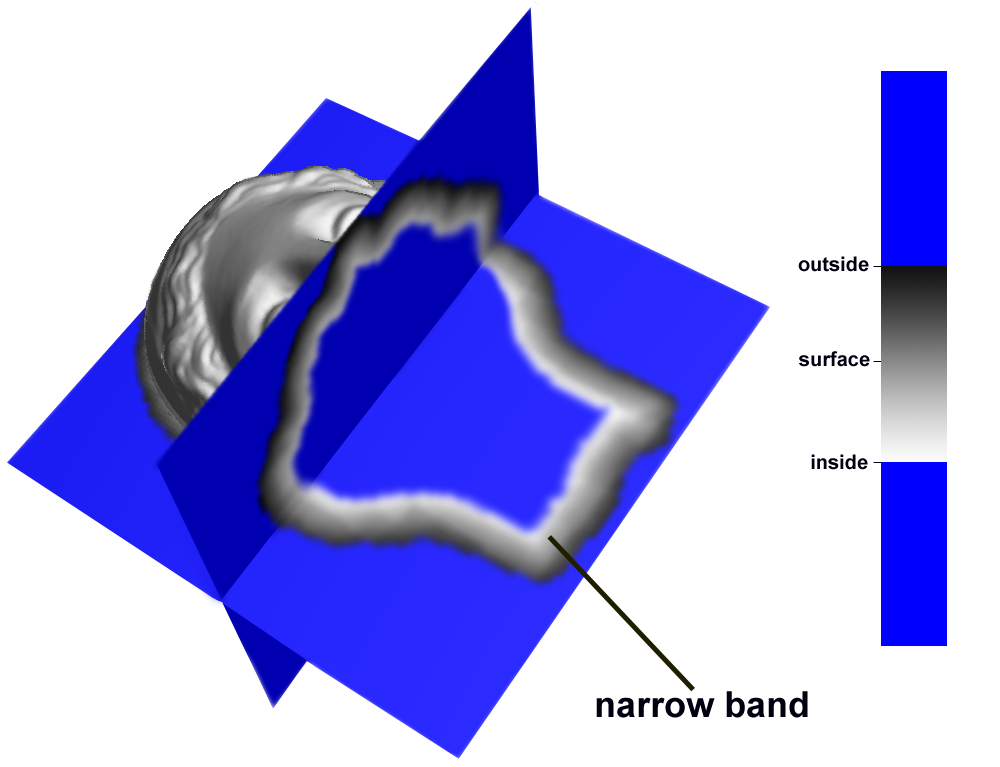
\includegraphics[width=0.3\textwidth]{figures/IgeaNarrowBand}} \hfill
	\subfigure[Caption second.]{\label{fig:test2}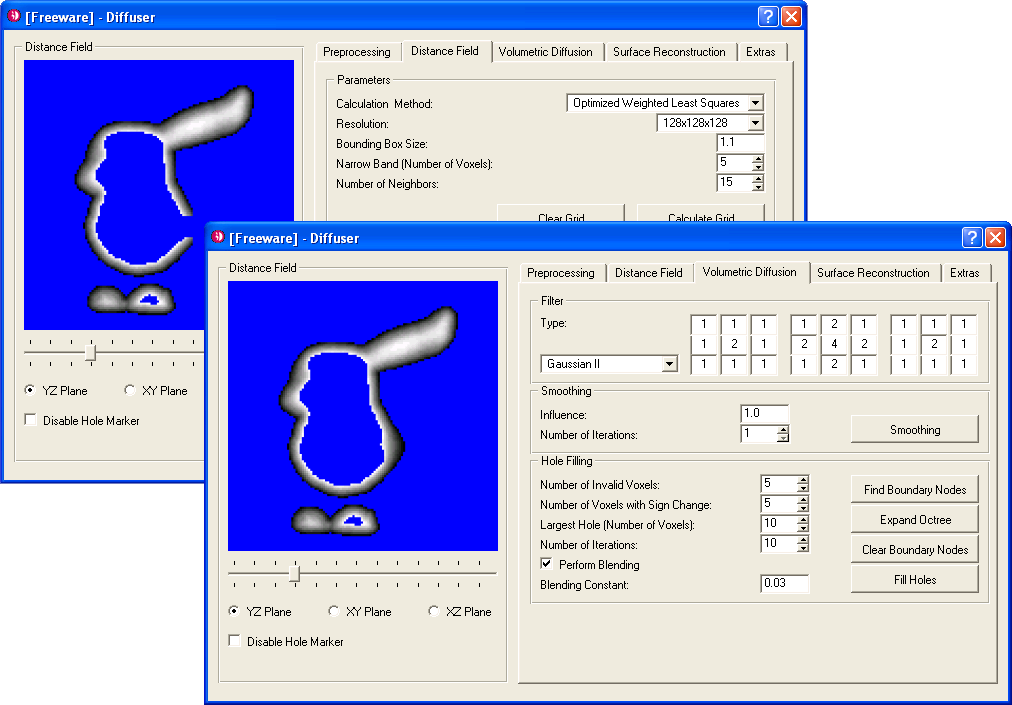
\includegraphics[width=0.3\textwidth]{figures/voldiff_ui}}
	\caption[Caption both]{Caption of both \subref{fig:test1}, \subref{fig:test2}.}
	\label{fig:bothfigures}
\end{figure}


Lorem ipsum dolor sit amet, consectetuer adipiscing elit, sed diam nonummy nibh euismod tincidunt ut laoreet dolore magna aliquam erat volutpat. Ut wisi enim ad minim veniam, quis nostrud exerci tation ullamcorper suscipit lobortis nisl ut aliquip ex ea commodo consequat. Duis autem vel eum iriure dolor in hendrerit in vulputate velit esse molestie consequat, vel illum dolore eu feugiat nulla facilisis at vero et accumsan et iusto odio dignissim qui blandit praesent luptatum zzril delenit augue duis dolore te feugait nulla facilisi. Lorem ipsum dolor sit amet, consectetuer adipiscing elit, sed diam 

\section{Second Section}

Lorem ipsum dolor sit amet, consectetuer adipiscing elit, sed diam nonummy nibh euismod tincidunt ut laoreet dolore magna aliquam erat volutpat. Ut wisi enim ad minim veniam, quis nostrud exerci tation ullamcorper suscipit lobortis nisl ut aliquip ex ea commodo consequat. Duis autem vel eum iriure dolor in hendrerit in vulputate velit esse molestie consequat, vel illum dolore eu feugiat nulla facilisis at vero et accumsan et iusto odio dignissim qui blandit praesent luptatum zzril delenit augue duis dolore te feugait nulla facilisi. Lorem ipsum dolor sit amet, consectetuer adipiscing elit, sed diam nonummy nibh euismod tincidunt ut laoreet dolore magna aliquam erat volutpat. Ut wisi enim ad minim veniam, quis nostrud exerci tation ullamcorper suscipit lobortis nisl ut aliquip ex ea commodo consequat. Duis autem vel eum iriure dolor in hendrerit in vulputate velit esse molestie consequat, vel illum dolore eu feugiat nulla facilisis at vero et accumsan et iusto odio dignissim qui blandit

% !TEX root = ../thesis.tex

\chapter{Conclusion and Outlook}

Lorem ipsum dolor sit amet, consectetuer adipiscing elit, sed diam nonummy nibh euismod tincidunt ut laoreet dolore magna aliquam erat volutpat. Ut wisi enim ad minim veniam, quis nostrud exerci tation ullamcorper suscipit lobortis nisl ut aliquip ex ea commodo consequat. Duis autem vel eum iriure dolor in hendrerit in vulputate velit esse molestie consequat, vel illum dolore eu feugiat nulla facilisis at vero et accumsan et iusto odio dignissim qui blandit praesent luptatum zzril delenit augue duis dolore te feugait nulla facilisi. Lorem ipsum dolor sit amet, consectetuer adipiscing elit, sed diam nonummy nibh euismod tincidunt ut laoreet dolore magna aliquam erat volutpat. Ut wisi enim ad minim veniam, quis nostrud exerci tation ullamcorper suscipit lobortis nisl ut aliquip ex ea commodo consequat. Duis autem vel eum iriure dolor in hendrerit in vulputate velit esse molestie consequat, vel illum dolore eu feugiat nulla facilisis at vero et accumsan et iusto odio dignissim qui blandit

Lorem ipsum dolor sit amet, consectetuer adipiscing elit, sed diam nonummy nibh euismod tincidunt ut laoreet dolore magna aliquam erat volutpat. Ut wisi enim ad minim veniam, quis nostrud exerci tation ullamcorper suscipit lobortis nisl ut aliquip ex ea commodo consequat. Duis autem vel eum iriure dolor in hendrerit in vulputate velit esse molestie consequat, vel illum dolore eu feugiat nulla facilisis at vero et accumsan et iusto odio dignissim qui blandit praesent luptatum zzril delenit augue duis dolore te feugait nulla facilisi. Lorem ipsum dolor sit amet, consectetuer adipiscing elit, sed diam nonummy nibh euismod tincidunt ut laoreet dolore magna aliquam erat volutpat. Ut wisi enim ad minim veniam, quis nostrud exerci tation ullamcorper suscipit lobortis nisl ut aliquip ex ea commodo consequat. Duis autem vel eum iriure dolor in hendrerit in vulputate velit esse molestie consequat, vel illum dolore eu feugiat nulla facilisis at vero et accumsan et iusto odio dignissim qui blandit
Lorem ipsum dolor sit amet, consectetuer adipiscing elit, sed diam nonummy nibh euismod tincidunt ut laoreet dolore magna aliquam erat volutpat. Ut wisi enim ad minim veniam, quis nostrud exerci tation ullamcorper suscipit lobortis nisl ut aliquip ex ea commodo consequat. Duis autem vel eum iriure dolor in hendrerit in vulputate velit esse molestie consequat, vel illum dolore eu feugiat nulla facilisis at vero et accumsan et iusto odio dignissim qui blandit praesent luptatum zzril delenit augue duis dolore te feugait nulla facilisi. Lorem ipsum dolor sit amet, consectetuer adipiscing elit, sed diam nonummy nibh euismod tincidunt ut laoreet dolore magna aliquam erat volutpat. Ut wisi enim ad minim veniam, quis nostrud exerci tation ullamcorper suscipit lobortis nisl ut aliquip ex ea commodo consequat. Duis autem vel eum iriure dolor in hendrerit in vulputate velit esse molestie consequat, vel illum dolore eu feugiat nulla facilisis at vero et accumsan et iusto odio dignissim qui blandit

Lorem ipsum dolor sit amet, consectetuer adipiscing elit, sed diam nonummy nibh euismod tincidunt ut laoreet dolore magna aliquam erat volutpat. Ut wisi enim ad minim veniam, quis nostrud exerci tation ullamcorper suscipit lobortis nisl ut aliquip ex ea commodo consequat. Duis autem vel eum iriure dolor in hendrerit in vulputate velit esse molestie consequat, vel illum dolore eu feugiat nulla facilisis at vero et accumsan et iusto odio dignissim qui blandit praesent luptatum zzril delenit augue duis dolore te feugait nulla facilisi. Lorem ipsum dolor sit amet, consectetuer adipiscing elit, sed diam nonummy nibh euismod tincidunt ut laoreet dolore magna aliquam erat volutpat. Ut wisi enim ad minim veniam, quis nostrud exerci tation ullamcorper suscipit lobortis nisl ut aliquip ex ea commodo consequat. Duis autem vel eum iriure dolor in hendrerit in vulputate velit esse molestie consequat, vel illum dolore eu feugiat nulla facilisis at vero et accumsan et iusto odio dignissim qui blandit



% ---- END MAIN PART ----


\appendix
\clearpage
\renewcommand*{\chapterpagestyle}{myappendixpagestyle}

% !TEX root = ../thesis.tex

\chapter{Information For The Few (Appendix)}

Nein, meine Texte les ich nicht, so nicht, st�hnte Oxmox. Er war mit Franklin, Rockwell und dem halbtaxgrauen Panther Weidemann in Memphis (Heartbreak Hotel) zugange. Sie warteten auf die fette Gill, um bei der Bank of Helvetica die Kapit�lchen in Kapital umzuwandeln. Oxmox liess nicht locker. Ich fleh euch an, rettet meine Copy, gebt meinem Body nochn Durchschuss! Kein Problem, erbarmte sich Old Face Baskerville, streichelte seinen Hund, zog seine einspaltige Poppl, legte an und traf! (Zeidank nichts Ernstes --- nurn bisschen Fraktur.) Oxmox: Danke, ist jetzt mit Abstand besser. Derweil jumpte der Fox leise over the Buhl, die sich mal wieder immerdar wie jedes Jahr gesellte. Diesmal war Guaredisch ihr Erw�hlter, weil seine Laufweite einem vollgetankten Bodoni entsprach und seine ungez�gelte Unterl�nge ihre Serifen so serafisch streifte, dass sie trotz Techtelmechtelei die magere Futura, jene zuverl�ssige und gern eingesetzte Langstreckenl�uferin, rechtsb�ndig �berholen konnten.

\section{Foo Bar Baz}

Nein, meine Texte les ich nicht, so nicht, st�hnte Oxmox. Er war mit Franklin, Rockwell und dem halbtaxgrauen Panther Weidemann in Memphis (Heartbreak Hotel) zugange. Sie warteten auf die fette Gill, um bei der Bank of Helvetica die Kapit�lchen in Kapital umzuwandeln. Oxmox liess nicht locker. Ich fleh euch an, rettet meine Copy, gebt meinem Body nochn Durchschuss! Kein Problem, erbarmte sich Old Face Baskerville, streichelte seinen Hund, zog seine einspaltige Poppl, legte an und traf! (Zeidank nichts Ernstes --- nurn bisschen Fraktur.) Oxmox: Danke, ist jetzt mit Abstand besser. Derweil jumpte der Fox leise over the Buhl, die sich mal wieder immerdar wie jedes Jahr gesellte. Diesmal war Guaredisch ihr Erw�hlter, weil seine Laufweite einem vollgetankten Bodoni entsprach und seine ungez�gelte Unterl�nge ihre Serifen so serafisch streifte, dass sie trotz Techtelmechtelei die magere Futura, jene zuverl�ssige und gern eingesetzte Langstreckenl�uferin, rechtsb�ndig �berholen konnten.

\section{Barontes}

Nein, meine Texte les ich nicht, so nicht, st�hnte Oxmox. Er war mit Franklin, Rockwell und dem halbtaxgrauen Panther Weidemann in Memphis (Heartbreak Hotel) zugange. Sie warteten auf die fette Gill, um bei der Bank of Helvetica die Kapit�lchen in Kapital umzuwandeln. Oxmox liess nicht locker. Ich fleh euch an, rettet meine Copy, gebt meinem Body nochn Durchschuss! Kein Problem, erbarmte sich Old Face Baskerville, streichelte seinen Hund, zog seine einspaltige Poppl, legte an und traf! (Zeidank nichts Ernstes --- nurn bisschen Fraktur.) Oxmox: Danke, ist jetzt mit Abstand besser. Derweil jumpte der Fox leise over the Buhl, die sich mal wieder immerdar wie jedes Jahr gesellte. Diesmal war Guaredisch ihr Erw�hlter, weil seine Laufweite einem vollgetankten Bodoni entsprach und seine ungez�gelte Unterl�nge ihre Serifen so serafisch streifte, dass sie trotz Techtelmechtelei die magere Futura, jene zuverl�ssige und gern eingesetzte Langstreckenl�uferin, rechtsb�ndig �berholen konnten.


\section{A Long Table with Booktabs}


{\scriptsize
\begin{longtable}{clccccccc}
\caption[Wordlist]{A sample list of words.}\\
\toprule
ID & Word & Word Length & WD & ETL & PTL &  WDplus \\
\midrule
\endfirsthead
\caption[]{(Continued)}\\
\toprule
ID & Word & Word Length & WD & ETL & PTL &  WDplus \\
\midrule
\endhead
\midrule
\multicolumn{9}{c}{continued on next page}\\
\bottomrule
\endfoot
%\bottomrule
\endlastfoot
\hline
1 & Eis & 3 & 4 & 0.42 & 1.83 & 0.19 \\ \hline
2 & Mai & 3 & 5 & 0.49 & 1.92 & 0.19 \\ \hline
3 & Art & 3 & 5 & 0.27 & 1.67 & 0.14 \\ \hline
4 & Uhr & 3 & 5 & 0.57 & 1.87 & 0.36 \\ \hline
5 & Rat & 3 & 5 & 0.36 & 1.71 & 0.14 \\ \hline
6 & weit & 4 & 6 & 0.21 & 1.65 & 0.25 \\ \hline
7 & eins & 4 & 6 & 0.38 & 1.79 & 0.26 \\ \hline
8 & Wort & 4 & 6 & 0.30 & 1.62 & 0.20 \\ \hline
9 & Wolf & 4 & 6 & 0.18 & 1.54 & 0.19 \\ \hline
10 & Wald & 4 & 6 & 0.31 & 1.63 & 0.19 \\ \hline
11 & Amt & 3 & 6 & 0.30 & 1.67 & 0.14 \\ \hline
12 & Wahl & 4 & 7 & 0.36 & 1.77 & 0.42 \\ \hline
13 & Volk & 4 & 7 & 0.45 & 1.81 & 0.20 \\ \hline
14 & Ziel & 4 & 7 & 0.48 & 1.78 & 0.42 \\ \hline
15 & vier & 4 & 7 & 0.38 & 1.81 & 0.42 \\ \hline
16 & Kreis & 5 & 7 & 0.26 & 1.62 & 0.33 \\ \hline
17 & Preis & 5 & 7 & 0.28 & 1.51 & 0.33 \\ \hline
18 & Re-de & 4 & 7 & 0.22 & 1.56 & 0.33 \\ \hline
19 & Saal & 4 & 7 & 0.75 & 2.10 & 0.43 \\ \hline
20 & voll & 4 & 7 & 0.48 & 1.82 & 0.24 \\ \hline
21 & weiss & 5 & 7 & 0.21 & 1.59 & 0.36 \\ \hline
22 & �r-ger & 5 & 7 & 1.16 & 2.69 & 0.59 \\ \hline
23 & bald & 4 & 7 & 0.18 & 1.56 & 0.19 \\ \hline
24 & hier & 4 & 7 & 0.40 & 1.70 & 0.43 \\ \hline
25 & neun & 4 & 7 & 0.17 & 1.52 & 0.26 \\ \hline
26 & sehr & 4 & 7 & 0.36 & 1.85 & 0.43 \\ \hline
27 & Jahr & 4 & 7 & 0.50 & 1.82 & 0.43 \\ \hline
28 & Gold & 4 & 7 & 0.04 & 1.35 & 0.20 \\ \hline
29 & T�-ter & 5 & 8 & 0.15 & 1.39 & 0.59 \\ \hline
30 & Tei-le & 5 & 8 & 0.30 & 1.71 & 0.46 \\ \hline
31 & Na-tur & 5 & 8 & 0.18 & 1.59 & 0.41 \\ \hline
32 & Feu-er & 5 & 8 & 0.30 & 1.71 & 0.45 \\ \hline
33 & Rol-le & 5 & 8 & 0.15 & 1.46 & 0.45 \\ \hline
34 & Rock & 4 & 8 & 0.29 & 1.68 & 0.25 \\ \hline
35 & Spass & 5 & 8 & 0.28 & 1.64 & 0.32 \\ \hline
36 & G�s-te & 5 & 8 & 0.49 & 1.75 & 0.66 \\ \hline
37 & En-de & 4 & 8 & 0.36 & 1.72 & 0.33 \\ \hline
38 & Kunst & 5 & 8 & 0.26 & 1.59 & 0.35 \\ \hline
39 & Li-nie & 5 & 8 & 0.45 & 1.88 & 0.63 \\ \hline
40 & B�u-me & 5 & 8 & 0.48 & 1.92 & 0.45 \\ \hline
41 & B�h-ne & 5 & 9 & 0.94 & 2.48 & 0.62 \\ \hline
42 & Bahn & 4 & 9 & 0.21 & 1.62 & 0.42 \\ \hline
43 & B�r-ger & 6 & 9 & 0.38 & 1.70 & 0.65 \\ \hline
44 & Druck & 5 & 9 & 0.60 & 2.03 & 0.31 \\ \hline
45 & zehn & 4 & 9 & 0.41 & 1.84 & 0.42 \\ \hline
46 & Va-ter & 5 & 9 & 0.36 & 1.78 & 0.40 \\ \hline
47 & Angst & 5 & 9 & 0.29 & 1.56 & 0.35 \\ \hline
48 & lei-der & 6 & 9 & 0.13 & 1.47 & 0.52 \\ \hline
49 & h�u-fig & 6 & 9 & 0.82 & 2.31 & 0.52 \\ \hline
50 & le-ben & 5 & 9 & 0.38 & 1.85 & 0.40 \\ \hline
51 & aus-ser & 6 & 9 & 1.20 & 2.26 & 0.57 \\ \hline
52 & be-vor & 5 & 9 & 1.28 & 2.75 & 0.39 \\ \hline
53 & Kai-ser & 6 & 9 & 0.92 & 2.37 & 0.53 \\ \hline
54 & Markt & 5 & 9 & 0.23 & 1.58 & 0.28 \\ \hline
55 & Os-ten & 5 & 9 & 0.21 & 1.54 & 0.48 \\ \hline
56 & Krieg & 5 & 9 & 0.33 & 1.67 & 0.50 \\ \hline
57 & Mann & 4 & 9 & 0.31 & 1.47 & 0.25 \\ \hline
58 & Hal-le & 5 & 9 & 0.24 & 1.65 & 0.45 \\ \hline
59 & heu-te & 5 & 9 & 0.44 & 1.87 & 0.46 \\ \hline
60 & in-nen & 5 & 10 & 0.36 & 1.80 & 0.45 \\ \hline
61 & Na-men & 5 & 10 & 0.28 & 1.72 & 0.41 \\ \hline
62 & jetzt & 5 & 10 & 0.70 & 2.07 & 0.32 \\ \hline
63 & kei-ner & 6 & 10 & 0.28 & 1.62 & 0.53 \\ \hline
64 & Schu-le & 6 & 10 & 1.02 & 2.12 & 0.48 \\ \hline
65 & Ar-beit & 6 & 10 & 0.34 & 1.70 & 0.52 \\ \hline
66 & An-teil & 6 & 10 & 0.27 & 1.63 & 0.53 \\ \hline
67 & di-rekt & 6 & 10 & 0.67 & 2.04 & 0.47 \\ \hline
68 & vor-her & 6 & 10 & 0.78 & 2.25 & 0.47 \\ \hline
69 & wol-len & 6 & 10 & 0.44 & 1.85 & 0.51 \\ \hline
70 & Kampf & 5 & 10 & 0.70 & 1.96 & 0.27 \\ \hline
71 & �n-dern & 6 & 10 & 1.18 & 2.62 & 0.65 \\ \hline
72 & lau-fen & 6 & 10 & 0.21 & 1.64 & 0.52 \\ \hline
73 & Eu-ro-pa & 6 & 10 & 0.23 & 1.53 & 0.66 \\ \hline
74 & statt & 5 & 10 & 1.61 & 2.86 & 0.39 \\ \hline
75 & Wes-ten & 6 & 10 & 0.29 & 1.60 & 0.54 \\
\bottomrule
\label{tab:wordlist}
\end{longtable}
}

\clearpage
\renewcommand*{\chapterpagestyle}{empty}

%\nocite{*}
\cleardoublepage
\phantomsection
\addcontentsline{toc}{chapter}{Bibliography}
\bibliography{graphics}

\end{document}
